% -*- TeX -*- -*- UK -*- -*- Soft -*-


\chapter{Server User Manual}
\label{chap:ServerUserManual}

\section{libraddask Template for Radiative Transfer}
\label{sec:libraddaskTemplateforRadiativeTransfer}

The User Manual is by way of example in using the \libraddask{} server.



This notebook tests the main functionality and demonstrates the use of the libraddask library.
The notebook  is available in the \lstinline{/libraddask/doc} folder as 
(\lstinline{libraddaskTemplate.ipynb}).

It calculates the radiative transfer calculations for the Sentinel 3 overpass over
Roodeplaat (\ang{25;37;29}S, \ang{28;21;39}E) on Sunday 2016-06-05.



\section{Running libRadtran}
\label{sec:RunninglibRadtran}

\begin{enumerate}
\item If working off-site, use a \ac{VPN} client to connect to the same network as used by the server.  Dask requires that your local PC must have an IP number in the same subnetwork as the server.  Some VPNs do not provide an IP number on the same subnetwork and such VPN clients will not work with Dask.
\item Using a remote terminal client on your local computer, open three terminal windows on the server:

\begin{itemize}
\item a  terminal for general use,
\item a terminal for the Dask scheduler, and
\item a terminal for the Dask workers.
\end{itemize}
\item In the scheduler terminal activate the conda environment with the Dask packages and then start the scheduler.

\begin{lstlisting}
conda activate mordevpy37
dask-scheduler
\end{lstlisting}
The scheduler responds with something like this:
\begin{lstlisting}[style=tinysize]
(base) dgriffith@nimbus:~$ conda activate mordevpy37        
(mordevpy37) dgriffith@nimbus:~$ dask-scheduler
distributed.scheduler - INFO - -----------------------------------------------
distributed.scheduler - INFO - Local Directory:    /tmp/scheduler-ay08oqkc
distributed.scheduler - INFO - -----------------------------------------------
distributed.scheduler - INFO - Clear task state
distributed.scheduler - INFO -   Scheduler at:  tcp://146.64.246.94:8786
distributed.scheduler - INFO -   dashboard at:                     :8787
\end{lstlisting}
   
Observe the scheduler URI: \lstinline{tcp://146.64.246.94:8786}, this must be used in the next step to set up the workers.

\item 
In the worker terminal change to the \verb+bin+ folder in the libRadtran installation folder and activate the conda environment with the Dask packages and then start the worker, using the scheduler URI and setting the required number of processors on the cluster :
\begin{lstlisting}
cd libRadtran/libRadtran-2.0.3/bin    
conda activate mordevpy37    
dask-worker tcp://146.64.246.94:8786 --nprocs 8
\end{lstlisting}
This should start eight workers, each with a different port number (not all detail shown below):
\begin{lstlisting}[style=tinysize]
(base) dgriffith@nimbus:~$ cd libRadtran/libRadtran\-2\.0\.3/bin        
(base) dgriffith@nimbus:~/libRadtran/libRadtran\-2\.0\.3/bin$ conda activate mordevpy37
(mordevpy37) dgriffith@nimbus:~/libRadtran/libRadtran-2.0.3/bin$ dask-worker tcp://146.64.246.94:8786 --nprocs 8
distributed.nanny - INFO -         Start Nanny at: 'tcp://146.64.246.94:33671'
distributed.nanny - INFO -         Start Nanny at: 'tcp://146.64.246.94:46725'
distributed.nanny - INFO -         Start Nanny at: 'tcp://146.64.246.94:42509'
distributed.nanny - INFO -         Start Nanny at: 'tcp://146.64.246.94:42983'
distributed.nanny - INFO -         Start Nanny at: 'tcp://146.64.246.94:43735'
distributed.nanny - INFO -         Start Nanny at: 'tcp://146.64.246.94:36947'
distributed.nanny - INFO -         Start Nanny at: 'tcp://146.64.246.94:40075'
distributed.nanny - INFO -         Start Nanny at: 'tcp://146.64.246.94:40495'
...
distributed.worker - INFO -       Start worker at:  tcp://146.64.246.94:36533
distributed.worker - INFO -          Listening to:  tcp://146.64.246.94:36533
distributed.worker - INFO -          dashboard at:        146.64.246.94:43069
distributed.worker - INFO - Waiting to connect to:   tcp://146.64.246.94:8786
distributed.worker - INFO - -------------------------------------------------
distributed.worker - INFO -               Threads:                          4
distributed.worker - INFO -                Memory:                    4.21 GB
distributed.worker - INFO -       Local Directory: /home/dgriffith/libRadtran/libRadtran-2.0.3/bin/dask-worker-space/worker-_0o0qta1
distributed.worker - INFO - -------------------------------------------------
distributed.worker - INFO -         Registered to:   tcp://146.64.246.94:8786
distributed.worker - INFO - -------------------------------------------------
distributed.core - INFO - Starting established connection
...
distributed.worker - INFO -       Start worker at:  tcp://146.64.246.94:46597
distributed.worker - INFO -          Listening to:  tcp://146.64.246.94:46597
distributed.worker - INFO -          dashboard at:        146.64.246.94:33737
distributed.worker - INFO - Waiting to connect to:   tcp://146.64.246.94:8786
distributed.worker - INFO - -------------------------------------------------
distributed.worker - INFO -               Threads:                          4
distributed.worker - INFO -                Memory:                    4.21 GB
distributed.worker - INFO -       Local Directory: /home/dgriffith/libRadtran/libRadtran-2.0.3/bin/dask-worker-space/worker-n0anjq00
distributed.worker - INFO - -------------------------------------------------
distributed.core - INFO - Starting established connection
distributed.worker - INFO -         Registered to:   tcp://146.64.246.94:8786
distributed.worker - INFO - -------------------------------------------------
distributed.core - INFO - Starting established connection
\end{lstlisting}
\item Run the code that activates the client in the local PC (see the code further down below). This should send the serialised data to the scheduler:
\begin{lstlisting}[style=tinysize]
distributed.scheduler - INFO - Register worker <Worker 'tcp://146.64.246.94:33437', name: tcp://146.64.246.94:33437, memory: 0, processing: 0>
distributed.scheduler - INFO - Starting worker compute stream, tcp://146.64.246.94:33437
distributed.core - INFO - Starting established connection
distributed.scheduler - INFO - Receive client connection: Client-1ed95fc0-8076-11ea-8700-cfd8862f98eb
distributed.core - INFO - Starting established connection
distributed.scheduler - INFO - Receive client connection: Client-27b067b0-8076-11ea-8700-cfd8862f98eb
distributed.core - INFO - Starting established connection
\end{lstlisting}
The scheduler will send the serialised data to the workers, which will execute the tasks:
\begin{lstlisting}[style=tinysize]
Running AerAng600to900nm
Running AerAng650to800nm
\end{lstlisting}

\end{enumerate}
If the libRadtran execution was successful the tasks should complete and the data returned to the client.

\section{Prepare for Python}


\begin{lstlisting}[style=tinysize]
import numpy as np
import matplotlib as mpl
import matplotlib.pyplot as plt
import datetime
import pytz
import copy # required for deepcopy

from dask.distributed import Client # For contacting the dask scheduler
import libraddask.rad.librad as librad

import pprint
pp = pprint.PrettyPrinter(indent=4)

%matplotlib inline
\end{lstlisting}


\section{Set up and Execute a Scenario or Case}
\label{sec:SetupandExecuteaScenarioorCase}

Populate an instance of the \lstinline{librad.Case} class.
Start with an empty instance and then add options to obtain the required input file for \libradtran{}.

Note that this code will be executed in the server's filesystem in\\
\lstinline{/home/dgriffith/libRadtran/libRadtran-2.0.3/bin/}\\
folder, so the paths must be relative to this executing location.  The paths defined here has no bearing to any folder on the local computer.



\begin{lstlisting}[style=tinysize]
# Create a blank libRadtran case
# with a name for this case
S3 = librad.Case(casename='AerAng600to900nm')

# Set revision
revision = '00A'

# Choose basic atmospheric profile
atmos_profile = '../data/atmmod/afglmw.dat'
# mid-latitude winter standard atmosphere
S3.set_option('atmosphere_file', atmos_profile)  

# Change to the Thuillier spectrum and set wavelength range appropriately
# these files must be present on the server, relative to the bin directory
solar_toa_file = '../data/solar_flux/Solar_irradiance_Thuillier_2002.txt'
solar_toa_file = '../data/solar_flux/kurudz_1.0nm.dat'

# Choose start and stop wavelengths and minimum edge margin in nm
wv_minimum_range = [[385.0, -2.0], [955.0, 2.0]]
S3.set_option('source solar', solar_toa_file)
S3.set_option('wavelength', 600.0, 900.0)

# Set up dates and times
# Overpass date and time down to second
overpass_datetime = datetime.datetime(2016, 6, 5, 7, 42, 31, tzinfo=pytz.utc)  
overpass_datestr = overpass_datetime.strftime('%Y%m%d')
# Get the day of year
day_of_year = int(overpass_datetime.strftime('%j'))

results_folder = 'ResultsS3on' + overpass_datestr + 'Rev' + revision

# Choose solver
S3.set_option('rte_solver disort')

# Set ground altitude
S3.set_option('altitude', 1.225)  # ground altitude in km above sea level

# Set ground albedo
S3.set_option('albedo 0.5')

# Set up aerosol model using the Angstrom law
S3.set_option('aerosol_default')
aot_wv = np.array([440, 500, 675, 870], dtype=np.float)  # MicroTOPS measurement wavelengths
aot = np.array([0.703, 0.615, 0.362, 0.206])  # MicroTOPS measurements
# Fit Angstrom law to data
alpha, beta = librad.angstrom_law_fit(aot_wv, aot)
# Fit King Byrne formula
alpha_0, alpha_1, alpha_2 = librad.king_byrne_formula_fit(aot_wv, aot)
S3.set_option('aerosol_angstrom', alpha, beta)

# Set up viewing and solar geometry. Note that these angles are taken from the S3 product and special
# care has to be taken when putting geometry information into libRadtran
OAA = 104.01066  # deg. Observation azimuth angle (presumably relative to north through east, satellite from dam)
OZA = 14.151356  # deg. Observation zenith angle (satellite zenith angle as seen from the dam)
SAA = 38.719933  # deg. Solar azimuth angle (presumably relative to north through east)
SZA = 59.316036  # deg. Solar zenith angle

S3.set_option('sza', SZA)  # deg. This one is straightforward
# Now when entering solar and observation zenith angles, it is necessary to provide the azimuth of light propagation
# rather than the azimuth of the view direction, which is 180 deg different
#S3.set_option('phi0', 180.0 - SAA)  # solar radiation propagation azimuth from north through east
#S3.set_option('phi', OAA)  # This is the azimuth of the satellite as seen from the target - also azimuth of light propgation
#S3.set_option('umu', np.cos(np.deg2rad(OZA))) # For downward-looking (upward propagating), check that umu is positive

S3.set_option('verbose')  # Will produce a lot of diagnostic output on stderr

#S3.set_option('zout boa')  # Set altitude of output data
S3.purge = False  # Prevent purging of output files

\end{lstlisting}


\begin{lstlisting}[style=tinysize]
# make a new case as a copy of existing
# If you use S3b = S3, both variables point to the same copy
# deepcopy operation required to create a new independent object

S3b = copy.deepcopy(S3)
# define a new spectral band, otherwise the same
S3b.name = 'AerAng650to800nm'
S3b.set_option('wavelength', 650.0, 800.0)
# S3b.set_option('aerosol_visibility', 5.0)
\end{lstlisting}


\begin{lstlisting}[style=tinysize]
#print out the current file contents
# Case().__repr__() provides the same output as written to the file.
print(f'S3:\n{S3}\n')
print(f'S3b:\n{S3b}\n')
\end{lstlisting}


\begin{lstlisting}[style=outcellstyle]
S3:
atmosphere_file ../data/atmmod/afglmw.dat
source solar ../data/solar_flux/kurudz_1.0nm.dat
wavelength 600.0 900.0
rte_solver disort
altitude 1.225
albedo 0.5
aerosol_default 
aerosol_angstrom 1.6848887536371142 0.18175118840581214
sza 59.316036
verbose 

\end{lstlisting}



\begin{lstlisting}[style=outcellstyle]
atmosphere_file ../data/atmmod/afglmw.dat
source solar ../data/solar_flux/kurudz_1.0nm.dat
wavelength 650.0 800.0
rte_solver disort
altitude 1.225
albedo 0.5
aerosol_default 
aerosol_angstrom 1.6848887536371142 0.18175118840581214
sza 59.316036
verbose 
\end{lstlisting}


\begin{lstlisting}[style=tinysize]
# create dask Client method with scheduler serverURI (IP and port)
serverURI = '146.64.246.94:8786'
client = Client(serverURI)

# count number of workers, obtained from scheduler
number_of_processes = len(client.scheduler_info()['workers'])
print(f'Number of workers: {number_of_processes}')
print(f'Client cores: {client.ncores()} ')

# uncomment to see the detail
# pp.pprint(client.get_versions(check=True))

\end{lstlisting}


\begin{lstlisting}[style=outcellstyle]
Number of workers: 8
Client cores: {'tcp://146.64.246.94:34397': 4, 'tcp://146.64.246.94:38009': 4, 'tcp://146.64.246.94:39663': 4, 'tcp://146.64.246.94:41169': 4, 'tcp://146.64.246.94:41399': 4, 'tcp://146.64.246.94:41797': 4, 'tcp://146.64.246.94:43815': 4, 'tcp://146.64.246.94:45191': 4} 

\end{lstlisting}


\begin{lstlisting}[style=tinysize]
# do a run on the server using two cases
futuresRad = client.map(librad.Case.run, [S3, S3b])
# Gather results. This will wait for completion of all tasks.
S3List = client.gather(futuresRad)    

# check the return values
librad.check_uvspec_run_success(S3List)
\end{lstlisting}


\begin{lstlisting}[style=outcellstyle]
All runs successful.

\end{lstlisting}


\begin{lstlisting}[style=tinysize]
# extract to 
S3 = S3List[0]
S3b = S3List[1]
\end{lstlisting}


\begin{lstlisting}[style=tinysize]
# Check for any errors by printing the return code and anything written to stderr
print(f'Return Codes : {S3.run_return_code} {S3b.run_return_code} ')
# print(f'Run({S3.name}) error (if any):\n{S3.stderr}')
# print(f'Run({S3b.name}) error (if any):\n{S3b.stderr}')
\end{lstlisting}


\begin{lstlisting}[style=outcellstyle]
Return Codes : 0 0 

\end{lstlisting}


\begin{lstlisting}[style=tinysize]
# now plot on the same graph
plt.figure(figsize=(16,9))
plt.plot(S3.wvl, S3.edn, S3b.wvl, S3b.edn)
plt.xlabel('Wavelength [nm]')
plt.ylabel('Irradiance [mW/m^2/nm]')
plt.title('Downwelling Spectral Irradiance')
plt.legend(['Spectral Range A', 'Spectral Range B'])
plt.grid()
# plt.savefig('ednAerAng.pdf')
\end{lstlisting}

\begin{center}
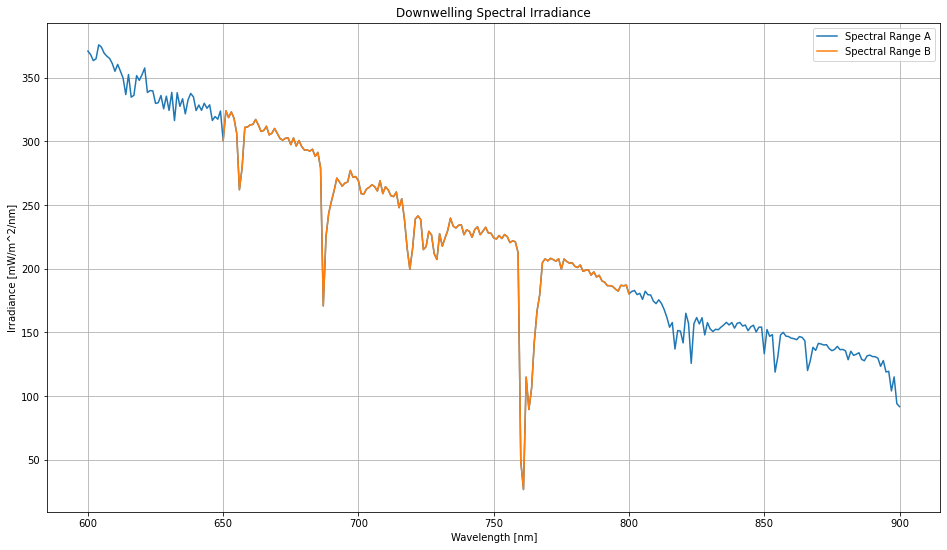
\includegraphics[width=0.6\textwidth]{./pic/libraddaskTemplate_14_0.png}
\end{center}


\section{Demonstrate King-Byrne and Angstrom Law}
\label{sec:DemonstrateKingByrneandAngstromLaw}

The run above was done using the Angstrom law parameters fitted to MicroTOPS measurements.




\begin{lstlisting}[style=tinysize]
# Check the quality of the Angstrom Law and King-Byrne formula fits
the_wv = np.arange(350.0, 950.0, 10.0)  # Pick a wavelength range
the_aot = librad.king_byrne_formula(the_wv, alpha_0, alpha_1, alpha_2)  # Calculate King-Byrne 
aot_ang = librad.angstrom_law(the_wv, alpha, beta)  # Calculate Angstrom Law
print(f'Angstrom alpha={alpha} beta={beta}')
print(f'king_byrne alpha0={alpha_0} alpha1={alpha_1} alpha2={alpha_2}')

\end{lstlisting}


\begin{lstlisting}[style=outcellstyle]
Angstrom alpha=1.6848887536371142 beta=0.18175118840581214
king_byrne alpha0=-1.9950667229251264 alpha1=-3.0186651652429806 alpha2=-1.2338155309188534

\end{lstlisting}


\begin{lstlisting}[style=tinysize]
# Set up atmospheric model and base case
atm = librad.Case(casename='RoodeplaatTransmittance')

# mid-latitude winter
atm.set_option('atmosphere_file', '../data/atmmod/afglmw.dat')  

# solar_toa_file = '../data/solar_flux/Solar_irradiance_Thuillier_2002.txt'
# solar_toa_file = '../data/solar_flux/kurudz_1.0nm.dat'
# atm.set_option('source solar', solar_toa_file)

# Choose solver
atm.set_option('rte_solver', 'disort')

# Set ground altitude (BOA) above sea-level
atm.set_option('altitude', 1.225)  # km AMSL

# Set up aerosol model
atm.set_option('aerosol_default')
# Aerosol type above 2km
# atm.set_option('aerosol_vulcan', 1)  
# Angstrom aerosol
atm.set_option('aerosol_angstrom', alpha, beta)

atm.set_option('wavelength', 400.0, 900.0)

SZA = 59.316036  # deg. Solar zenith angle
atm.set_option('sza', SZA)  # deg. This one is straightforward
atm.set_option('output_quantity transmittance')
atm.purge = False  # Prevent purging of output files

\end{lstlisting}


\begin{lstlisting}[style=tinysize]
print(f'atm:\n{atm}')
\end{lstlisting}


\begin{lstlisting}[style=outcellstyle]
atm:
atmosphere_file ../data/atmmod/afglmw.dat
rte_solver disort
altitude 1.225
aerosol_default 
aerosol_angstrom 1.6848887536371142 0.18175118840581214
wavelength 400.0 900.0
sza 59.316036
output_quantity transmittance

\end{lstlisting}


\begin{lstlisting}[style=tinysize]
# do a run on the server using two cases
futuresRad = client.map(librad.Case.run, [atm])

# Gather results. This will wait for completion of all tasks.
T3List = client.gather(futuresRad)    

# check the return values
librad.check_uvspec_run_success(T3List)
\end{lstlisting}


\begin{lstlisting}[style=outcellstyle]
All runs successful.

\end{lstlisting}

For some unknown reason the transmittance from libRadtran comes out significantly \textbf{smaller} than what the Angstrom equation predicts.



\begin{lstlisting}[style=tinysize]
T3a = T3List[0]
transm = T3a.edir[0:,0]
scaling = 3
txm = transm * scaling
\end{lstlisting}


\begin{lstlisting}[style=tinysize]
# Plot transmittance
plt.figure(figsize=(16,9))
plt.plot(the_wv, np.exp(- aot_ang))
plt.plot(the_wv, np.exp(- the_aot))
plt.plot(T3a.wvl, txm)
plt.xlabel('Wavelength [nm]')
plt.ylabel('Transmittance')
plt.title('Transmittance')
plt.legend(['Angstrom','King-Byrne',f'libRadtran, scaled by {scaling}'])
plt.grid()

\end{lstlisting}

\begin{center}
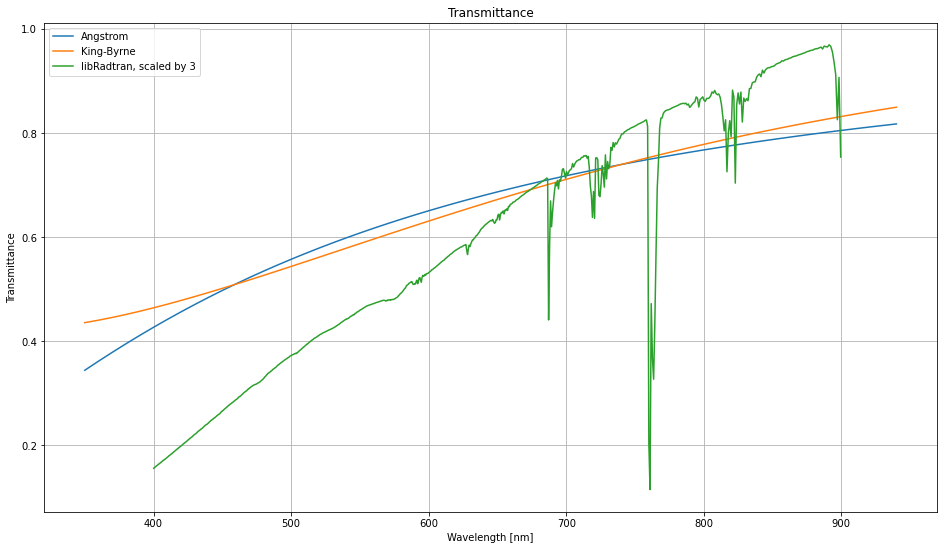
\includegraphics[width=0.6\textwidth]{./pic/libraddaskTemplate_22_0.png}
\end{center}


\begin{lstlisting}[style=tinysize]
# Plot Angstrom Law and King-Byrne fitted curves with MicroTOPS measurements
plt.figure(figsize=(16,9))
plt.plot(the_wv, the_aot, the_wv, aot_ang, aot_wv, aot, 'o')
plt.plot(T3a.wvl, -np.log(txm) )
plt.xlabel('Wavelength [nm]')
plt.ylabel('Aerosol Optical Thicknes')
plt.title('Aerosol Optical Thickness, Angstrom Law and King-Byrne Fit')
plt.legend(['King-Byrne', 'Angstrom', 'MicroTOPS',f'libRadtran, scaled by {scaling}'])
plt.grid()

\end{lstlisting}

\begin{center}
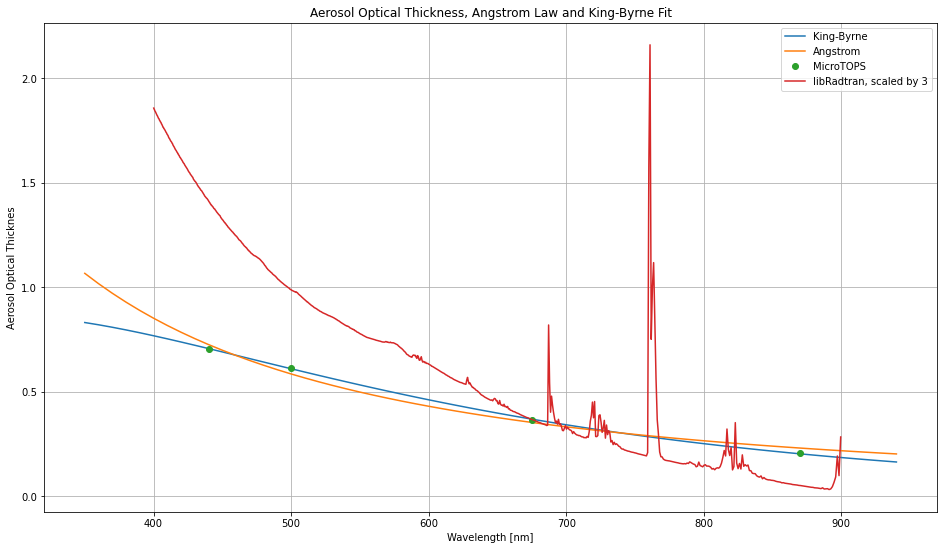
\includegraphics[width=0.6\textwidth]{./pic/libraddaskTemplate_23_0.png}
\end{center}


\section{Split Case}
\label{sec:SplitCase}

\verb+librad.Case()+ has the option to split a wavelength range into smaller sections.
These smaller sections can be executed on the server in parallel and the results merged afterwards.



\begin{lstlisting}[style=tinysize]
# Split up into number of sub-cases depending on the number of cores and 
# other factors on the compute cluster
# use wavelength overlap of 1.0 nm
atm_list = atm.split_case_by_wavelength(number_of_processes, overlap=1.0)  

# Take a look at the splits
print('file contents:')
print(atm_list[0],end='\n\n')

print(f'Spectral ranges for {number_of_processes} processes:')
for i,item in enumerate(atm_list):
    print(f"process {i} range={item.tokens[item.options.index('wavelength')]}")
\end{lstlisting}


\begin{lstlisting}[style=outcellstyle]
file contents:
atmosphere_file ../data/atmmod/afglmw.dat
rte_solver disort
altitude 1.225
aerosol_default 
aerosol_angstrom 1.6848887536371142 0.18175118840581214
wavelength 400.0 462.5
sza 59.316036
output_quantity transmittance

Spectral ranges for 8 processes:
process 0 range=['400.0', '462.5']
process 1 range=['461.5', '525.0']
process 2 range=['524.0', '587.5']
process 3 range=['586.5', '650.0']
process 4 range=['649.0', '712.5']
process 5 range=['711.5', '775.0']
process 6 range=['774.0', '837.5']
process 7 range=['836.5', '900.0']

\end{lstlisting}


\begin{lstlisting}[style=tinysize]
# run the list of spectral ranges
futureRadBatch = client.map(librad.Case.run, atm_list)
atm_listrtn = client.gather(futureRadBatch) 
# check the return values
librad.check_uvspec_run_success(atm_listrtn)
\end{lstlisting}


\begin{lstlisting}[style=outcellstyle]
All runs successful.

\end{lstlisting}


\begin{lstlisting}[style=incellstyle]
# Merge results for edir, which will be direct (specular) transmittance 
# in 'output transmittance' mode
wvl_atm_reptran, atm_reptran = \
    librad.Case.merge_caselist_by_wavelength(atm_listrtn, 'edir')

\end{lstlisting}


\begin{lstlisting}[style=tinysize]
# Plot transmittance
plt.figure(figsize=(16,9))
plt.plot(wvl_atm_reptran, atm_reptran)
plt.xlabel('Wavelength [nm]')
plt.ylabel('Transmittance')
plt.title('Transmittance of merged run data')
plt.grid()

\end{lstlisting}

\begin{center}
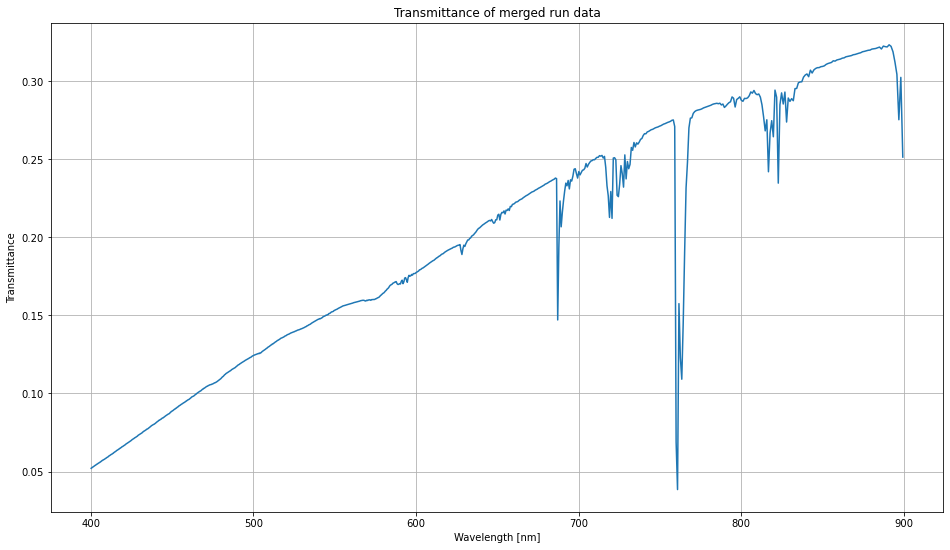
\includegraphics[width=0.6\textwidth]{./pic/libraddaskTemplate_28_0.png}
\end{center}


\section{Shutting down the Client}
\label{sec:ShuttingdowntheClient}

When the client is no longer required, shut it down.


BUT: this also kills the scheduler and/or workers!



\begin{lstlisting}[style=tinysize]
# client.shutdown()
\end{lstlisting}


\begin{lstlisting}[style=tinysize]
# to get software versions
# https://github.com/rasbt/watermark
# An IPython magic extension for printing date and time stamps, version numbers, and hardware information. 
# you only need to do this once
# !pip install watermark

%load_ext watermark
%watermark -v -m -p numpy,matplotlib,datetime,pytz,dask,dask.distributed,libraddask -g 
\end{lstlisting}


\begin{lstlisting}[style=outcellstyle]
CPython 3.7.6
IPython 7.13.0

numpy 1.18.1
matplotlib 3.2.1
datetime unknown
pytz 2019.3
dask 2.12.0
dask.distributed 2.12.0
libraddask 0.1.1

compiler   : MSC v.1916 64 bit (AMD64)
system     : Windows
release    : 7
machine    : AMD64
processor  : Intel64 Family 6 Model 94 Stepping 3, GenuineIntel
CPU cores  : 8
interpreter: 64bit
Git hash   : 678c42400523b7d730d6646132e271a7cacd8ab4

\end{lstlisting}


